\documentclass[12pt,a4paper]{report}
\usepackage[margin=20mm]{geometry}
% \usepackage{subfig}
\usepackage{fancyhdr}
\usepackage{lastpage}
\usepackage{parskip}
\usepackage{titlesec}
\usepackage{color}
\usepackage{listings}
\usepackage{moresize}
\usepackage{lipsum}
\usepackage{caption}
\usepackage{subcaption}
% \captionsetup{compatibility=false}
\usepackage{float}
\usepackage{graphicx}
\usepackage{upquote}
\usepackage{silence}


\usepackage[T1]{fontenc}
\usepackage[utf8]{inputenc}
\usepackage[scale=0.9]{sourcecodepro}

\usepackage{hyperref}
\hypersetup{
    colorlinks=false, %set true if you want colored links
    linktoc=all,     %set to all if you want both sections and subsections linked
    linkcolor=blue,  %choose some color if you want links to stand out
}

\captionsetup[figure]{width=0.8\textwidth,labelfont=sc,textfont={it}}
\captionsetup[table]{width=0.8\textwidth,labelfont=sc,textfont={it}}
\captionsetup[lstlisting]{width=0.8\textwidth,labelfont=sc,textfont={it}}


\lstset{
  basicstyle=\small\ttfamily,
  columns=fullflexible,
  breaklines=true,
  % numbers=left,
  upquote=true,
  keywordstyle=\bfseries,
  basicstyle=\ttfamily,
  numberstyle=\tiny,
  numbersep=20pt,
  tabsize=3,
  escapeinside={@}{@}, 
}

\renewcommand\labelitemi{--}


%\titleformat{\chapter}\normalfont\LARGE\bfseries}{Chapter \thechapter \newline }{1em}{}

%  \titleformat{\chapter}[hang]{\Huge\bfseries}{\thechapter\hsp\color{gray}{|}\hsp}{0pt}{\Huge\bfseries}

%\titleformat{\chapter}{ \huge \sc \bfseries}{\thechapter.}{0.5em}{}\titlespacing\chapter{0pt}{12pt plus 4pt minus 2pt}{0pt plus 2pt minus 2pt}

\definecolor{gray75}{gray}{0.5}
\newcommand{\hsp}{\hspace{20pt}}

%\titleformat{\chapter}[hang]{\Huge\bfseries}{\textcolor{gray75}{Chapter \thechapter} \hsp \textcolor{gray75}{|}\hsp}{0pt}{\Huge \sc\bfseries}

%\titleformat{\chapter}[hang]{\Huge\bfseries}{\textcolor{gray75}{Chapter \thechapter}\hsp \textcolor{gray75}{---}\hsp}{0pt}{\Huge \sc \bfseries}[{\color{gray75}\titlerule[0.1pt]}]

\titleformat{\chapter}[hang]{\Huge\bfseries}{\textcolor{gray75}{Chapter \thechapter}\hsp \textcolor{gray75}{---}\hsp}{0pt}{\sc \bfseries}
% [{\color{gray75}\titlerule[1pt]}]
%\titlespacing\chapter{0pt}{-4em}{0pt}
\titlespacing{\chapter}{0pt}{0pt}{0pt}



%\titleformat{\section}{ \huge \sc \bfseries}{\thesection.}{0.5em}{}
%\titlespacing\section{0pt}{12pt plus 4pt minus 2pt}{0pt plus 2pt minus 2pt}

\titleformat{\section}
{ \Large  \bfseries}{\thesection}{0.5em}{}
\titlespacing\section{0pt}{12pt plus 4pt minus 2pt}{0pt plus 2pt minus 2pt}

\titleformat{\subsection}
{\bfseries\large}{\thesubsection}{0.5em}{}
\titlespacing\subsection{0pt}{12pt plus 4pt minus 2pt}{0pt plus 2pt minus 2pt}


\newcommand{\name}{Phoebe Nichols}
\newcommand{\crsid}{pmn29}


\newcommand{\minih}[1]{\textbf{#1} \vspace{0.1em} \\}

\pagestyle{fancy}


\renewcommand{\headrulewidth}{0pt}
\cfoot{\thepage\ of \pageref{LastPage}}
\lhead{ \emph \normalfont \leftmark}
\rhead{ \emph \normalfont \rightmark}

\setlength{\headheight}{15pt}


%For chapter headings
\fancypagestyle{normal}{%
\cfoot{\thepage\ of \pageref{LastPage}}
% \lhead{ \emph \normalfont \leftmark}
% \rhead{ \emph \normalfont \rightmark}

\lhead{\leftmark }

}

%For chapter headings
\fancypagestyle{plain}{%
\lhead{}
\rhead{}
  %\fancyfoot[C]{\thepage\ of \pageref{LastPage}}%
  %\renewcommand{\headrulewidth}{0pt}% Line at the header invisible
  %\renewcommand{\footrulewidth}{0.4pt}% Line at the footer visible
}

%For chapter headings
\fancypagestyle{none}{%
\lhead{}
\rhead{}
\cfoot{}
}


\renewcommand\labelitemi{--}

\begin{document}

% Stuff to do:
% Signpost 
% Repeat key points 
% Include a summary of each chapter

\pagestyle{none}

\rightline{\Large \bfseries Phoebe Nichols}

\vspace*{60mm}
\begin{center}
{\Huge  \bfseries An Implementation of Prolog} \\[5mm]
{\Large Computer Science Tripos -- Part II \\[5mm]
Churchill College}
\end{center}

\newpage
\pagestyle{normal}

\tableofcontents



% Datalog and emerging applications: An interactive tutorial.
% In SIGMOD, pages 1213–1216, 2011.



\chapter{Introduction}

\section{Project summary}

TODO

\section{Motivation}

\subsection{Declarative programming}

Declarative programming languages are a family of programming language that describe logical properties of the result of a computation, but do not specify how the computation should be performed. This is in contrast to imperative programming languages, which describe a sequence of commands for the computer to perform. Logic programming languages are a class of declarative programming languages where the program consists of a series of logical statements describing the result of the program.

 The motivation for logic programming is that it provides a useful layer of abstraction: the idea is that the programmer's life should be simplified if they need only be concerned with the logic associated with their program. {\color{red}  is this achieved in practice? seem like it is not, prolog not popular} Although logic programming languages are not the most popular {\color{red} why? }, they have some important applications. Examples of these applications include:
 \begin{itemize}
\item Datalog is a subset of Prolog that is used as a database query language. This language has modern applications in 
data integration, declarative networking, program analysis, information extraction,
network monitoring, security, and cloud computing \cite{datalog}. {\color{red} why is datalog good for this?} For example, the Doop framework uses Datalog for points-to analysis of Java programs \cite{doop}.

\item 
Prolog has been used in the JVM 11 specification  provide a formal description of semantics of the JVM \cite{jvm11}.

\item {\color{red} some standard AI application for prolog? hihi hi hi}


 \end{itemize}

 % The most popular logic programming language is Prolog {\color{red} source?} 

% The motivation for declarative programming over procedural programming is that declarative programming provides a higher level of abstraction: the declarative programmer only needs concern herself with logical statements describing the result of a computation. 

% In computer science, declarative programming is a programming paradigm—a style of building the structure and elements of computer programs—that expresses the logic of a computation without describing its control flow.




- Motivation for project

\section{Related work}

The first logic programming language was called Baroque, and was implemented in 1972. This was an  assembly-like language that used logical statements in the form of Horn clauses \cite{Kowalski2002}. The first Prolog system was also implemented in 1972, by Alain Colmerauer and Philippe Roussel. They chose the name Prolog as an abbreviation for `programmation en logique' (meanning programming in logic).
 Robert Kawalski and Maarten van Emden then formalised the use of predicate logic as a programming language \cite{kowalski},\cite{logprog}.

 This early work on Prolog was followed by David Warren's invention of the Warren Abstract Machine \cite{WAM}. This is an abstract machine for the efficient execution of Prolog, and is used by popular Prolog execution systems such as SWI-Prolog \cite{REFswi}.



Mycroft, Mercury

% Back in Marseilles, Roussel
% and Colmerauer designed and implemented the first
% Prolog system in Algol-W as an adaptation of Roussel’s
% existing SL-resolution theorem prover. Teaming with
% Pasero they implemented a large natural language pro-
% cessing system. This was the first major program writ-
% ten in Prolog [6], and it was written in 1972. I

% Kowalski, R.A. The predicate calculus as a programming language.
% In Proceedings of the Internafional Symposium and Summer School on
% Mathematical Foundations of Computer Science (Jablonna, Poland,
% Aug.). 1972.

%  Colmerauer, A., Kanoui, H., Pasero, R., and Roussel, P. Un systeme
% de communication
%  homme-machine
%  an FranGais. Rep., Groupe
% d’Intelligence Artificielle,
%  Univ. d’Aix Marseille II. Luminy, France.
% 1973.


% Maarten van Emden and Robert Kowalski defined a set of semantics for predicate logic as a programming language \cite{logprog}. This paper described the basis of logic programming. 

% \cite{logprog}

% % van Emden, M. and Kowalski, R., "The Semantics of Predicate Logic as a Programming Language", in Journal of the ACM, Vol. 23, No. 4, 1976, pp. 733–742.

% the first Prolog system was developed in 1972 by Colmerauer and Phillipe Roussel

% - Discuss previous related work

% - How the work fits into the broader area of Computer Science




% The name Prolog was chosen by Philippe Roussel as an abbreviation for programmation en logique (French for programming in logic). It was created around 1972 by Alain Colmerauer with Philippe Roussel, based on Robert Kowalski's procedural interpretation of Horn clauses. It was motivated in part by the desire to reconcile the use of logic as a declarative knowledge representation language with the procedural representation of knowledge that was popular in North America in the late 1960s and early 1970s. According to Robert Kowalski, the first Prolog system was developed in 1972 by Colmerauer and Phillipe Roussel.[5] The first implementation of Prolog was an interpreter written in Fortran by Gerard Battani and Henri Meloni. David H. D. Warren took this interpreter to Edinburgh, and there implemented an alternative front-end, which came to define the “Edinburgh Prolog” syntax used by most modern implementations. Warren also implemented the first compiler for Prolog, creating the influential DEC-10 Prolog in collaboration with Fernando Pereira. Warren later generalised the ideas behind DEC-10 Prolog, to create the Warren Abstract Machine. 


% 26 marks for intro + prep = 3600 words
\chapter{Preparation} 

This chapter contains a discussion of the preparatory work done for each of the components of the project. It begins by discussing Prolog's features, execution model, and program structure. The Warren Abstract Machine is discussed---this is a common target for Prolog compilers---followed by an introduction to the Mycroft-OKeefe type system for Prolog. After the introduction of these concepts, preparatory work relating to the software engineering practice used  is explained, including a discussion of testing strategy and development methodology. The chapter finishes with a quick summary of its key points.

\section{Programming in Prolog}


A Prolog program is a set of Horn clauses. Each rule is a horn clause: a disjunction of literals with at most one positive literal. A search is performed over these horn clauses to try to derive the given query.

\subsection{Structure of a Prolog Program}

A Prolog program is comprised of a set of predicates, followed by a query. Each predicate is made up of at least one clause, and each clause has a head containing a list of argument terms and a body containing a list of calls to predicates. These concepts are described in more detail below.

\begin{description}

\item[Terms]
Prolog's only data structure is the term. A term is either an unbound variable, or a compound term consisting of a name and a (possibly empty) list of terms.

\item[Goals]
A goal consists of a predicate name and a list of argument terms to the predicate. When Prolog executes a goal, it searches for an interpretation of the argument terms  that satisfies the predicate.

\item[Clauses] Clauses represent logical statements that are true in the world described by the Prolog program. 
Each clause is a fact or a rule: 
\begin{itemize}
\item 
A fact consists of a predicate name and a list of argument terms; the meaning of a fact is that it defines the given instance of the relation as being true.

\item 
A rule consists of a head and a body. The head is a predicate name and a list of argument terms. The body is a non-empty list of goals. The meaning of a rule is that if we can show all the goals in the body are true then we can derive that the head is true.
\end{itemize}

\item[Predicates]
A predicate is defined by the set of clauses with the same name and arity. A goal for a predicate can be derived from any of the clauses of the predicate, but the clauses are tried in the order that they are found in the program.

\item[Queries]
A query is a list of goals that are to be derived by the Prolog program, and a Prolog program has at most one query. 
% A substitution to the variables in the query such that the query can be derived is returned from the execution of a program. 
The execution of a program is a search for a substitution to the variables in the query that gives a satisfying interpretation for all the goals in the query; the result of the execution is either such an interpretation, failure, or an infinite loop.


\end{description}

\section{The execution mechanism of Prolog}

{\color{red} what order of logic is prolog}

{\color{red}
simple summary

Somewhere: clause precidence!


depth first search}

\subsection{Linear resolution}

% SLD resolution (Selective Linear Definite clause resolution) is the basic inference rule used in logic programming. It is a refinement of resolution, which is both sound and refutation complete for Horn clauses. 


% SLD-resolution is a special case of a refinement of
% the resolution method due to Kowalski and Kuehner known as SL-resolution
% (Kowalski and Kuehner, 1970)

% Linear resolution with selection function (SL-resolution) is a restricted form of linear resolution. The main restriction is effected by a selection function which chooses from each clause a single literal to be resolved upon in that clause. This and other restrictions are adapted to linear resolution from Loveland's model elimination.

Resolution is an inference rule that combines two complementary literals. A statement of resolution in {\color{red} prepositional} logic is 
\begin{equation}
\frac{\neg A \rightarrow B \qquad B \rightarrow C}{\neg A \rightarrow C}
\label{resolution}
\end{equation}
Linear resolution is a technique for first order logic theorem proving where resolution is repeatedly applied, with each resolvent being used as a parent clause for the next resolutions step.

{\color{red} give substitution rule}

% The proof has a linear structure: each
% % resolvent becomes the parent clause for the next resolution
% step. Furthermore, the other parent clause is always one
% of the original set of clauses. This simple structure is very
% efficient because only the last resolvent needs to be saved.
% It is similar to the execution strategy of Prolog.




The basic execution mechanism of Prolog uses SLD (Simple Linear Definite Clause) resolution; a definite clause is a Horn clause with at most one positive literal. This is a special form of linear resolution for Horn clauses based on Kuehner and  Kowalski's SL-resolution \cite{Kowalski1971}---this performs linear resolution using a selection function to choose the literal to be resolved. In the case of SLD resolution, one of the literals to be resolved is the head of a clause and the other is a member of the body of a clause.

 % SLD resolution is a term used in logic programming to refer to the control strategy used in such languages to resolve issues of nondeterminism. By definition, SLD resolution is linear resolution with a selection function for definite sentences. A definite sentence has exactly one positive literal in each clause and this literal is selected to be resolved upon, i.e., replaced in the goal clause by the conjunction of negative literals which form the body of the clause. 

 

\subsection{Unification}
% Unification is the operation of finding a common instance
% of two or more terms. 


Unification is the operation of finding a {\color{red} minimal?} substitution that gives the same resultant term when applied to a pair of possibly-distinct terms $(A,B)$. A substitution is a mapping from the variables in a term to terms that replace these variables when the substitution is applied. In order for a goal to be derived using the resolution rule given in equation \ref{resolution} the goal must be unified with the head of some clause. It is through this process of unification that Prolog variables are instantiated.

Unification is the basic operation of Prolog. When a clause \texttt{clause1(t1,...,tn) :- body.} is called with arguments \texttt{a1,...,an}, each \texttt{ti} is unified with \texttt{ai} before the body calls are performed. Here, `calling' a clause corresponds to performing resolution with the clause. The individual Prolog terms unify as follows:
\begin{itemize}

\item The unification of a variable with any other term succeeds and binds the value of the variable to the value of the other term. 

\item Compound terms unify if their top function symbol and arity are the same and their lists of arguments unify recursively. It should be noted that these lists of argument terms might be empty.


\end{itemize}

\subsection{Search strategy}

Prolog performs a depth-first, left-to-right search for the solution to a query: when trying to derive a list of goals, the first goal must be derived before Prolog progresses to the second goal. It is important that a logic programming language specify its search strategy because the same program may give a different ordering of results when it is executed with various search strategies {\color{red} example program?}. 
There are advantages to other search strategies over depth first search: breadth first search will always find a solution if one exists, whereas depth first search may get stuck in a loop. 

% It is possible to use other search strategies for 


% - BFS has better termination properties

% - DFS

% - Backtracking

% - Parallelism?


\subsection{Cut}

Cut, written \texttt{!}, is a predicate that  may be found in the body of a clause. The effect of a cut is to:
\begin{enumerate}
\item Commit to the current clause, meaning that no other clause from the same predicate will be backtracked to within this call to the predicate.
\item And discard all choice points created by executing goals inside the current clause up until the cut.
\end{enumerate}

Cut is known as an extra-logical predicate because it does not have a declarative reading. Cut is, however, useful for improving the efficiency of Prolog programs since cut can prevent unnecessary backtracking. Cut also increases the expressivity of Prolog, for example cut can be used to implement logical negation.

\subsection{Negation}

It was relevant to understand negation in Prolog to understand if this was a feature that I should implement. Negation can be implemented using cut and so I decided that it was not a core feature for a Prolog compiler and therefore did not choose to implement it.

In Prolog, cut provides negation . This is demonstrated by the following example of using cut to define a \texttt{not\_unify} clause:
\begin{lstlisting}
unify(X,X).

not_unify(A,B) :- unify(A,B), !, fail.
not_unify(A,B).
\end{lstlisting}
This program uses the \texttt{fail} predicate: this is simply a predicate that always fails to be derived.

\section{The Warren Abstract Machine}

% The Warren Abstract Machine is the best thing to happen to humanity since sliced bread and American cheese. Known by those who love it as the WAM, it's as easy as peanuts to simulate Prolog using the l33t hax first proposed by my boy Warren.

The Warren Abstract Machine (WAM) was designed by David Warren in 1983 \cite{WAM} and has become the standard target for Prolog compilers. It defines an instruction set that can be efficiently interpreted, and serves as a useful intermediate representation when compiling Prolog to native code. 

\subsection{Variable representation}

An important feature of the WAM is that it represents variables as pointers. The unification of a variable with a structure is therefore implemented by making the variable point to the representation of the structure in memory. Similarly, the unification of two variables is represented by making one variable point to the other. Multiple applications of unification can lead to the creation of chains of pointers.

{\color{red} wam variable binding higher lower trailing rule?}

{\color{red} link to discussion of aliasing problem}

\subsection{Instructions}

The WAM instruction set contains five main types of instruction:
\begin{enumerate}
\item \emph{Get} instructions, used to fetch a procedure's arguments from a standard location. {\color{red} where do I define procedure?}
\item \emph{Put} instructions, used to load the arguments to a procedure into a standard location. 
\item \emph{Unify} instructions, used to perform unification. These instructions verify that two terms have the same structure, and unify variables within the terms to enforce this property. 
\item \emph{Procedural} instructions, used for control transfer and environment allocation for procedure calls.
\item \emph{Indexing} instructions, used to link the different clauses making up a procedure.
\end{enumerate}
These instructions are interpreted by the WAM, in the same way as Java byte-code instructions are interpreted by the JVM.

\subsection{Memory areas }

The WAM has three main areas of memory: the local stack, heap, and trail stack.
\begin{enumerate}  
\item The  \emph{local stack} contains environments and choice points. Environments contain the state associated with the call to a predicate: they are similar to stack frames on traditional architectures. Choice points contain the information needed to backtrack to an earlier point in the computation.

\item The  \emph{heap} contains structures and lists created by unification; these are pointed to by variables in the stack.

\item The \emph{trail stack} contains references to variables that were bound on unification. These references are stored so that they can be unbound on backtracking. 
\end{enumerate}

{\color{red} + detail}

% \subsection{Structure sharing vs structure copying}

% \subsection{Representation of unification}

\section{The Mycroft-OKeefe type system}

The Mycroft-OKeefe type system \cite{mycroftTypes} is a polymorphic type system for Prolog, based on the Hindley-Milner type system. Type definitions in this type system consist of a type name--possibly associated with a list of type variables--followed by a list of different type constructors for this type, possibly each using the type variables. Type declarations are needed for each predicate, and the types of variables are inferred. Figure \ref{mlvsmyc} compares an implementation of append in ML to an implementation using the Mycroft-OKeefe type sytem.


\begin{figure}
\centering 
\small 

\begin{subfigure}{0.7\linewidth}
\begin{lstlisting}[frame=tb]
datatype 'a list = Cons of 'a * 'a list | Nil

fun append(x,Nil) = Cons(x,Nil)
| append(x,Cons(y,z)) = Cons(y,append(x,z))
\end{lstlisting}
\subcaption{Append program in ML}
\end{subfigure}

\begin{subfigure}{0.7\linewidth} \hspace{1em}
\begin{lstlisting}[frame=tb]
type list A = cons(A,list(A)), nil.

pred append(B, list(B), list(B)).
append(X,nil,cons(X,nil)).
append(X,cons(Y,Z),cons(Y,Res)) :- append(X,Z,Res).
\end{lstlisting}

\subcaption{Append program in Prolog using the Mycroft-OKeefe type system}
\end{subfigure}

\WarningsOff
\captionsetup{type=lstlisting} 
\caption{Comparison between an append function implemented in ML and using the   Mycroft-OKeefe type system}
\label{mlvsmyc}
\end{figure}

\subsection{Type rules?}

\section{Evaluation strategy}

\section{Choice of tools}

% \begin{description}
% \item[OCaml] \lipsum[1-2]
% \end{description}


\subsection{OCaml}
I chose to implement my project in OCaml. There are a number of reasons for this decision:
% \begin{itemize}
% \item \emph{Lexer and parser generator tools} \\
% OCaml has good implementations of the standard lexer and parser generator tools \texttt{lex} and \texttt{yacc}, called \texttt{Ocamllex} \cite{ocamlyacc} and \texttt{Menhir} \cite{ocamlBook}. It was useful to use these tools instead of implementing a lexer and parser from scratch, particularly because the grammar was modified throughout the development of the project.


% \item \emph{Library support} \\ 
% There is good library support for OCaml, both from its standard library library and from external libraries such as the Jane Street core library. For this project, the Jane Street core library was used extensively to provide performant implementations of standard data-types.


% \item \emph{Static type checking and parametric polymorphism} \\ 
% OCaml's type system facilitates rapid development thanks to its type system. Parametric polymorphism means functions work across multiple data-types without any extra effort, and static type checking allows many program errors to be detected at compile time.


% \item \emph{Garbage collection} \\ 
% Having a garbage collector is useful in general because the programmer need not be concerned with memory management. Garbage collection is particularly useful for this project because the abstract machine implementation can use OCaml's garbage collector implicitly {\color{red} eval this? talk about why we want to garbage collect prolog?}


% \item \emph{Pattern matching} \\ 
% OCaml includes pattern matching syntax: this syntax has been used throughout the project, from walking the parse tree to driving the abstract machine. The project code would have taken longer to write and been more difficult to understand without this useful syntax.

% \item \emph{Familiarity with ML} \\ 
% I am familiar with ML from the IA course `Foundations of Computer Science'. OCaml is a member of the ML family  

% \end{itemize}

\begin{description}
\item[Lexer and parser generator tools]
OCaml has good implementations of the standard lexer and parser generator tools \texttt{lex} and \texttt{yacc}, called \texttt{Ocamllex} \cite{ocamlyacc} and \texttt{Menhir} \cite{ocamlBook}. It was useful to use these tools instead of implementing a lexer and parser from scratch, particularly because the grammar was modified throughout the development of the project.

\item[Library support]
There is good library support for OCaml, both from its standard library library and from external libraries such as the Jane Street core library. For this project, the Jane Street core library was used extensively to provide performant implementations of standard data-types.


\item[Static type checking and parametric polymorphism]
OCaml's type system facilitates rapid development thanks to its type system. Parametric polymorphism means functions work across multiple data-types without any extra effort, and static type checking allows many program errors to be detected at compile time.


\item[Garbage collection]
Having a garbage collector is useful in general because the programmer need not be concerned with memory management. Garbage collection is particularly useful for this project because the abstract machine implementation can use OCaml's garbage collector implicitly {\color{red} eval this? talk about why we want to garbage collect prolog?}


\item[Pattern matching]
OCaml includes pattern matching syntax: this syntax has been used throughout the project, from walking the parse tree to driving the abstract machine. The project code would have taken longer to write and been more difficult to understand without this useful syntax.

\item[Familiarity with ML]
I am familiar with ML from the IA course `Foundations of Computer Science'. OCaml is based on ML and has many similar features, so I have been able to learn the language quickly.

\end{description}

\subsection{Lexer and parser generators}

As mentioned above, the lexer and parser generators \texttt{Ocamllex} and \texttt{Menhir} were used. There was no alternative to \texttt{Ocamllex}, but an alternative to \texttt{Menhir} is \texttt{Ocamllyac} \cite{ocamlyacc}. \texttt{Menhir} was chosen because it has the advantage of generating more comprehensible error methods \cite{ocamlBook}.

% The biggest advantage of Menhir is that its error messages are generally more human-comprehensible, and the parsers that it generates are fully reentrant and can be parameterized in OCaml modules more easily. We recommend that any new code you develop should use Menhir instead of ocamlyacc.

% - OCaml


% -Ocamllex

% -Menhir

\subsection{OUnit}

The OCaml unit test framework \texttt{OUnit} \cite{OUnit} was used to write tests for the project. This was chosen because it is simple and well-documented; I could find example code matching my use-cases easily.

\section{Starting point}

The starting point given in my project proposal is copied below.

\fbox{
    \parbox{\textwidth}{ \setlength{\parskip}{0.5em}
    \vspace{-1.5em}
\subsection*{Prolog as a programming language}

I will need a good understanding of how to program in Prolog in order to implement the Prolog compiler. I will also need to write test programs for the subset of Prolog that I have chosen to compile. These tests will help me to evaluate the correctness and performance of my compiler and abstract machine implementation.

I am studying the 50\% course, which does not cover Prolog until Lent term this year. I have, therefore, studied the Prolog course over the summer.

\subsection*{Prolog compilation and execution}

I have no prior experience with implementing Prolog interpreters or compilers. The IB 75\%/II 50\% Prolog course that I studied over the summer introduced me to the basics of Prolog execution. I have also read around this area over the summer: some of the papers I read are cited in this document. I have not previously implemented any part of a Prolog compiler, interpreter, or abstract machine.

\subsection*{OCaml}

I am intending to implement all of my project in OCaml initially, although I may add some SWI-Prolog for extension features. I have chosen OCaml because I have experience implementing lexers and parsers in ML from the compilers course, and found ML convenient for this sort of thing. OCaml will have the same advantages as ML, but is more widely used and therefore has more tools and libraries available.

I have very little prior experience with OCaml (only from the IB compilers course), so I will need to dedicate time to studying it. This time is provisioned in my project plan.

% - Declare the starting point

% - What new things had to be learnt?
}
}


\section{Requirements analysis}

It is important to define the requirements of a project, both so that crucial features can be focussed on and to provide a means of assessing whether the project has been a success. The core requirements for my project is to implement the following components for a basic subset of Prolog:
\begin{itemize}
\item A lexer and parser should be implemented, either manually or using tools to generate these automatically.
\item A translator from the parse tree to byte-code should be implemented.
\item Abstract machine to execute this byte-code should be implemented. This abstract machine is indented to use a similar instruction set to the WAM, but does not need to implement all of its features.
\end{itemize}
There is no requirement concerning the performance of this system, but its performance should be evaluated and discussed in the evaluation section.


\section{Software engineering techniques}

- What is your software engineering technique? 

\subsection{Testing strategy}

\hrulefill

- Describe word undertaken before code written

- Show how project proposal was refined and clarified 


\section{Summary}

A summary of the key points in this chapter is given below.
\begin{itemize}
\item A Prolog program consists of a set of clauses followed by a query. Each clause is a statement in first order logic: writing a clause in a Prolog program is like saying to the Prolog interpreter `this statement holds'. Prolog performs a depth-first search over the clauses of a program to look for a satisfying interpretation for a given query; the result of a Prolog program is either a satisfying interpretation to the given query, failure, or an infinite loop.

\item  The Warren Abstract Machine is a common target for Prolog compilers. It defines abstract instruction set for Prolog that can be efficiently interpreted, similarly to how the JVM interprets Java byte-code.

\item Prolog can be typed using the Mycroft-OKeefe type system; this is a polymorphic type system similar to that of ML.

\item The project was implemented in OCaml, using automated lexer and parser generator tools. This decision
was made because OCaml has many desirable properties for this project, including: these good lexer and parser generator tools, static type checking, parametric polymorphism, pattern matching, good library support, garbage collection, and my prior familiarity with ML. 

\item A blahblah development methodology was used to blahblah
\end{itemize}

% 40 marks for implementation = 5600 words
\chapter{Implementation}

\section{Overall structure}

The overall pipeline of my project is given in figure \ref{pipeline}.

\begin{figure}
\begin{center}
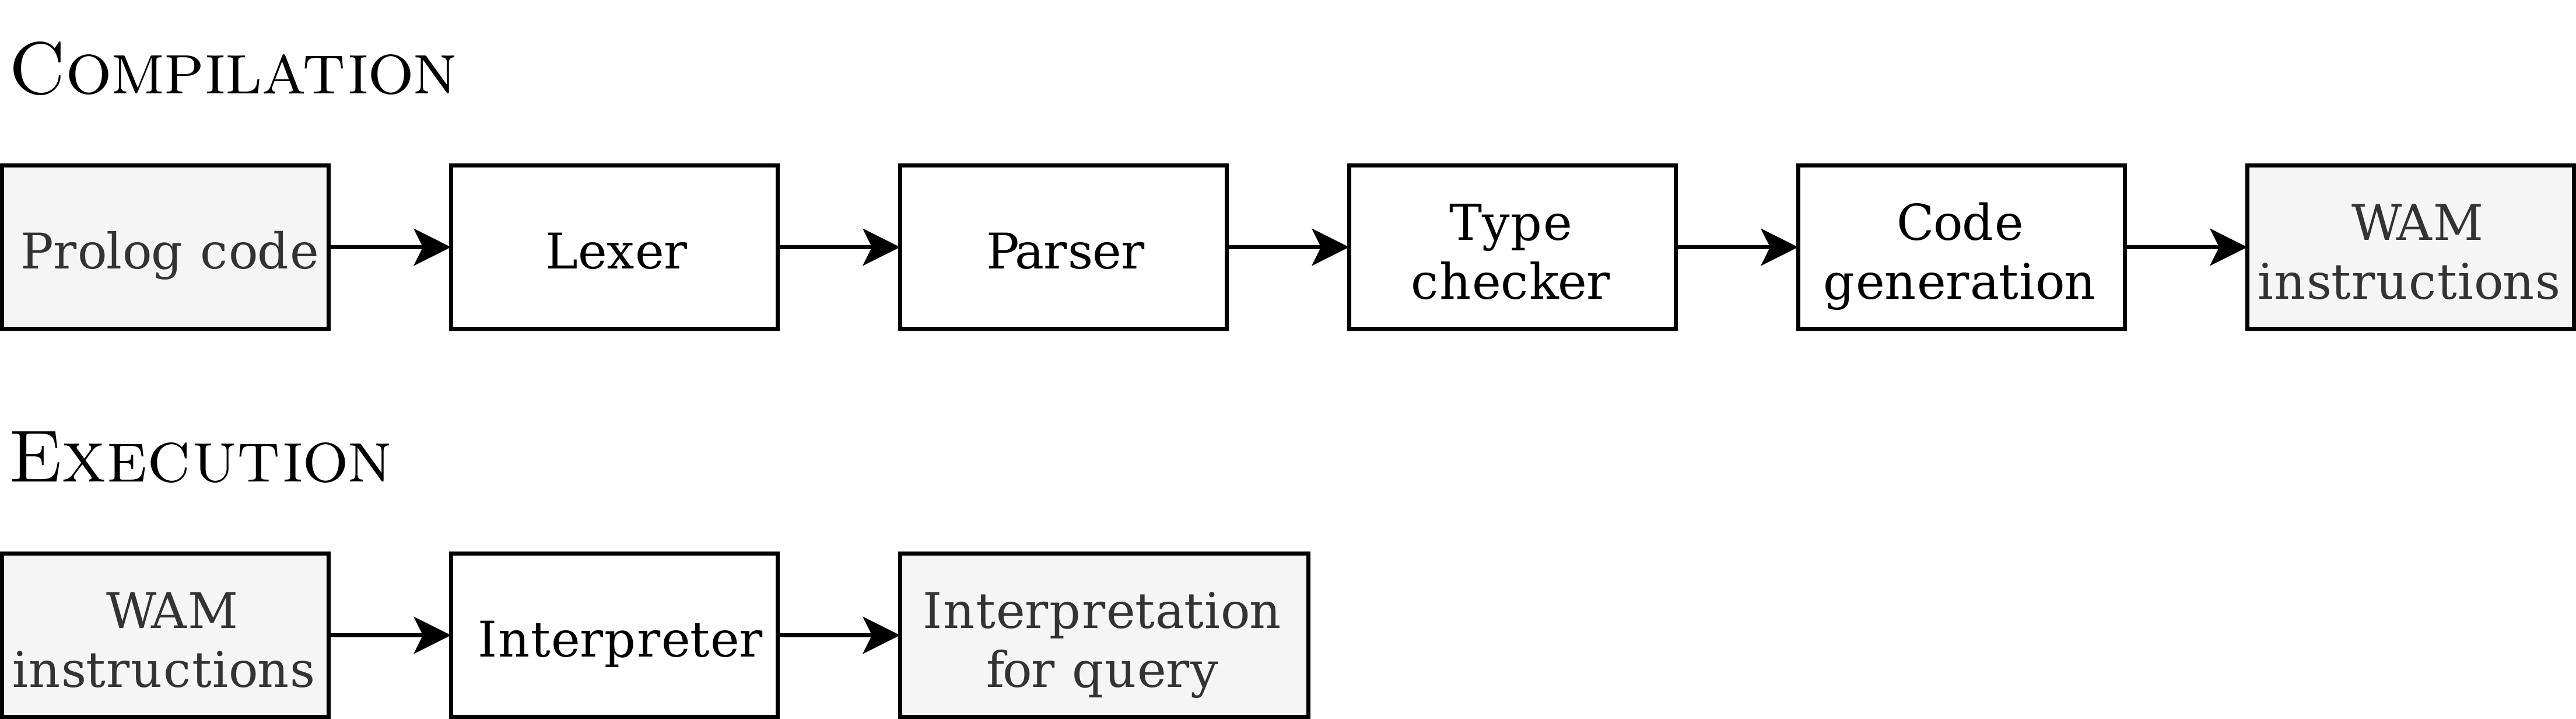
\includegraphics[width=0.9\linewidth]{diagrams/Pipeline.png}
\end{center}
\caption{Project pipeline}
\label{pipeline}
\end{figure}

\section{Lexer and parser}

The lexer and parser were implemented using the tools  \texttt{ocamllex}  \cite{ocamlyacc} and \texttt{menhir} \cite{ocamlBook}. {\color{red} useful for iterative development methodology}

% was implemented using the lexer-generator \texttt{ocamllex}  \cite{ocamlyacc}.


% The parser was implemented using the parser-generator \texttt{menhir} \cite{ocamlBook}.

\section{Initial interpreter}

\subsection{Variable representation}

\section{Abstract machine}

\subsection{Variable representation}

\section{Code generation}

\subsection{The instruction set}

- Actual instruction set?

\section{Code optimisation}

\subsection{Last call optimisation}

\subsection{Using type information}

\section{Code execution}

- Data structures used?

\subsection{Stack representation}

\section{Design strategy}

- Design strategy (does it look ahead to testing)

\section{Repository overview}

- Repository overview - describe high level structure of your source code 

\hrulefill 

- Describe what was produced

- Aliasing problem somewhere


\section{Summary}


% 20 marks for evaluation + conclusion = 2800 words
\chapter{Evaluation} 

Try to explain the results instead of just stating them

\section{Success criterion}

- Show project was a success

- How many of the original goals were achieved? -> were they proved to have been achieved

\section{Compiler correctness}

- Sample output

\section{Speed}

- Compare to other prologs 

- How effective were optimisations?

\section{Memory use}

- Compare to other prologs

\subsection{Last call optimisation}

\section{Performance gains from optimisation}

\section{Parallelisation?} 


\section{How to improve performance}

Where does most memory go?

Where does most time go?

\hrulefill 
    
- Show an ambitious case

- Tables of benchmark programs

- Graphs need confidence levels 


\section{Summary}

\chapter{Conclusions}

- Short 

- Summary

- Text-




\bibliographystyle{unsrt}

% \bibliographystyle{plain}

\bibliography{references}

\end{document}
